\documentclass[12pt]{article}
\usepackage{amssymb,amsmath}
\usepackage[pdftex]{graphicx}
\usepackage{epsfig,subfigure}
\usepackage{epstopdf}
\usepackage{bm,url}
\DeclareGraphicsExtensions{.jpg,.pdf,.png,.eps,.ps}
\usepackage[usenames, dvipsnames]{color}
\usepackage{appendix}
\usepackage{ulem}

\textheight = 522pt
\textwidth = 450pt

\oddsidemargin 0.0in

\newcommand{\Comment}[1]{\textcolor{Blue}{(Comment: #1)}}

\newcommand{\exec}{{Executive Team}}
\newcommand{\shorte}{{ET}}  %abbrev for \exec

%% Define a new 'leo' style for the package that will use a smaller font.
\makeatletter
\def\url@leostyle{%
  \@ifundefined{selectfont}{\def\UrlFont{\sf}}{\def\UrlFont{\small\ttfamily}}}
\makeatother
%% Now actually use the newly defined style.
\urlstyle{leo}

\begin{document}

\title{CMB-S4 Science Collaboration Bylaws}
\maketitle


\tableofcontents

%\Comment{ADD COMMENTS WITH $\backslash$Comment\{ \} }

\newpage


%\section{Collaboration Governance Objectives/Preamble}
\section{Preamble}

The purpose of the CMB-S4 Science Collaboration (hereafter the Collaboration) is to conduct a science program centered on the future Stage-4 ground-based cosmic microwave background (CMB) experiment, CMB-S4. The Collaboration activities include advocating for, and advancing the design of, CMB-S4. The Collaboration is expected to play a major role in the establishment of the CMB-S4 Construction Project (hereafter the Project) and in its operations, and the Collaboration is expected to lead the scientific analysis. 
%construction and operation of the future Stage-4 %experiment that is intended to be the definitive 
CMB-S4 will deliver a highly constraining data set with which any model for the origin of the primordial fluctuations---be it inflation or an alternative theory---and their evolution to the structure seen in the Universe today must be consistent. 
This document outlines the Collaboration governance and organization of scientific activities.

\subsection{Collaboration Governance Objectives}
 The structure of the Collaboration was designed to adhere to the following principles:

\begin{itemize}
\item The Collaboration organization will be based on models used in other successful  large DOE- and NSF-supported experiments.  %Cosmic Frontier 

\item The Collaboration will strive to maximum the scientific return of the experiment, producing high-quality science in a timely manner and promoting full utilization of the data through public data releases after a suitable proprietary period.

\item The organizational structure of the Collaboration will enable broad representation of its Members, and encourage consensus in decision making. %while fostering 

\item   All Members of the Collaboration will be expected to contribute to the success of the Collaboration and the Project through work on one or more areas of necessary infrastructure. The organizational structure should incentivize Collaboration Members to contribute to the advancement of CMB-S4 including work on hardware, software, testing, commissioning, operations, common science infrastructure, documentation,  publications,  management tasks and serving in leadership roles.

%\item All Members of the collaboration will be expected to contribute to the success of the project through work on one or more areas of necessary infrastructure.

\item Towards this end, the Collaboration should provide appropriate credit to data analysts and builders of hardware and/or software; provide leadership opportunities and other opportunities to promote career advancement; motivate people to work together towards common goals; %to complete the key project deliverables; 
and provide a healthy collaboration culture that establishes standards for behavior consistent with high ethical standards.

\end{itemize}


\subsection{Definitions}

The CMB-S4 Construction Project (the Project) is distinct from the CMB-S4 Science Collaboration (the Collaboration). The Project will be responsible for final design and construction of CMB-S4, which by necessity will have strong oversight and  report directly to the associated funding agencies and other sources of funding.  The Collaboration and Project must work closely together; many Collaboration Members are expected to have important roles within the Project. The Project ends when construction is completed and operations begin. Operations may be the responsibility of the Collaboration, or may be conducted by a distinct entity working closely with the Collaboration. These Bylaws pertain only to the Science Collaboration and do not specify the structure of, or relationship to, the Project or Operations. 
\vskip 12pt


Throughout this document,  a ``supermajority vote" is defined as a result with more than two-thirds of the votes received in favor of  the motion. \textcolor{red}{``Supermajority votes'' require approval by two-thirds of the entire voting body.} A ``majority vote" requires that more than half the votes received are in favor of the motion.   A ``quorum" for a meeting is defined as the presence of a majority of a body's members.   For collaboration-wide votes, a ``Voting Member" is  defined as a Senior Member or a Postdoctoral Member (see \S\ref{sec:memberrights}). ``Ex officio" Members of a governance body are those whose membership is owing to their roles elsewhere in the Collaboration.  For example, the Science Council Chairs (\S\ref{sec:SC}) are ex officio Members of the Executive Team (\S\ref{sec:exec}).  In these bylaws,  ``Working Groups" are open to all Collaboration Members, and ``Councils" have multiple Working Groups reporting to them, while ``Committees" do not.  

 %The presence of a simple majority of a body's members constitutes quorum for a meeting, and two-thirds of a body must be present for a vote to be valid.

%Add definition of �ex officio� membership as membership by virtue of having another role, so that the Science Council Chairs are ex officio members of the ET,  and when a new Chair is elected, the old Chair rolls off the ET. 



\section{Overall Structure}
The governance structure of the CMB-S4 Collaboration  is illustrated in Figure~\ref{fig:org_chart}.  The Governing Board (GB) provides oversight to an \exec\ (ET) led by two equal co-Spokespersons.  A number of Councils, Committees and Working Groups carry out necessary work to enable the overall science objectives of the Collaboration. The overall scope, selection of, and interplay among these governance entities is described in the remainder of this document. 


\begin{figure}[h!]
\begin{center}
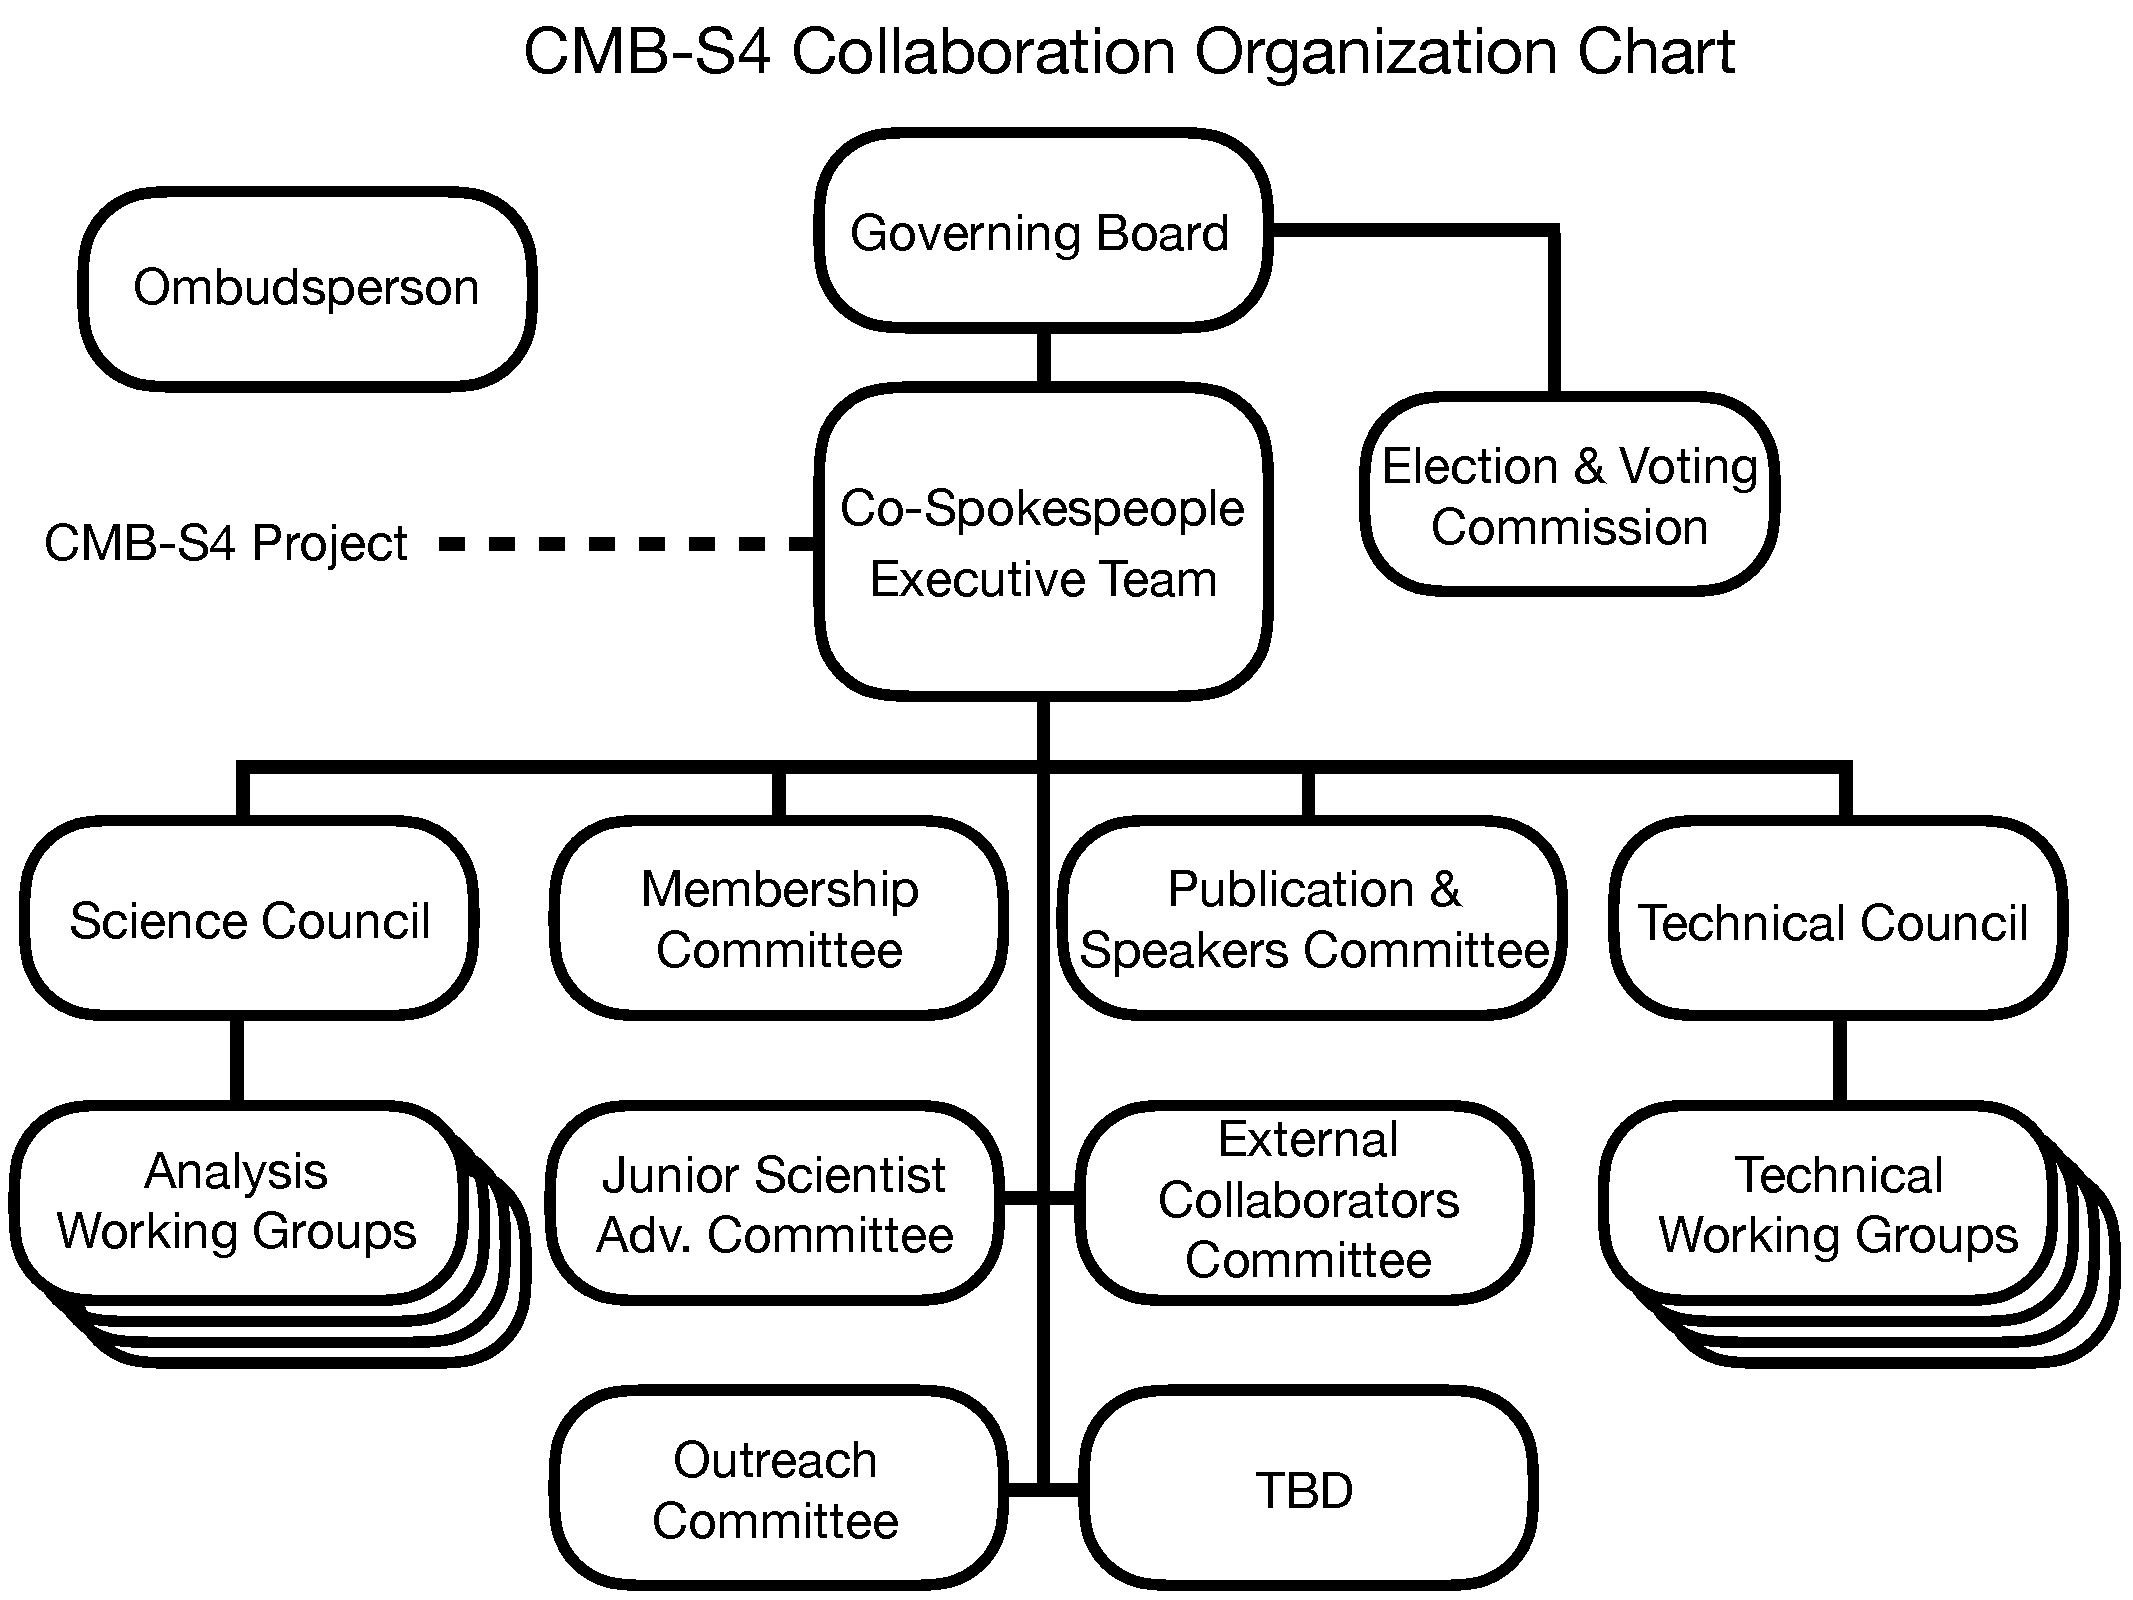
\includegraphics[width=6.5in]{CMB-S4_Org_chart_+_details_v9.pdf}
\end{center}
\caption{CMB-S4 Collaboration Organizational Chart}
\label{fig:org_chart}
\end{figure}

\section{Governing Board}

The Governing Board (GB), a body whose composition is designed to be representative of the membership of the Collaboration as a whole, is the %ultimate 
policy forming body of the Collaboration.  Its other key role is oversight of the Spokespersons and the \exec.

\subsection{Scope}
%The Governing Board has two main roles: to facilitate discussion of collaboration-wide issues---especially those that concern the self-governance of the CMB-S4 Collaboration---and to provide oversight of the Spokespersons and the \exec. %and the co-spokepersons.
Any powers not explicitly assigned to a different governing body in these Bylaws reside in the Governing Board.
Governing Board responsibilities include, but are not limited to:  %omitted "Collaboration as a whole---

\begin{itemize}
\item Oversight of the overall progress, status and functioning of the Collaboration.  

\item Oversight of the Spokespersons and their activities.  The GB charges the Spokespersons to prepare a yearly plan for the Collaboration.  The plan must be ratified by a supermajority vote of the GB.  The GB charges the Spokespersons to carry out specific duties for the Collaboration, including, but not limited to, Collaboration reviews, and reviews of the Councils and Committees operating under the auspices of the Spokespersons and the \exec.  The GB may require a detailed verbal, or written report from the Spokespersons on any action. The GB may remove a Spokesperson by a supermajority vote if their performance is insufficient. %See also \S\ref{sec:removal}.

%\item Charging the Spokepersons to carry out specific duties for the collaboration, including, but not limited to, collaboration reviews, committee, and board reviews. 

%\item Charging the Spokepersons with preparation of a yearly plan for the collaboration and the ratification of this plan. 

\item Approval and revision of Collaboration Bylaws, including the Membership and Publication and Speakers policies.   Amendment of the Bylaws requires a supermajority of the GB.  Major changes (see \S\ref{subsec:amend}) must be ratified by the Voting Members of the Collaboration.  %This excludes any Bylaws that directly pertain the power, scope, election, etc. of the GB, which will be discussed in Section \ref{subsec:amend}.


%\item Oversight of the activities of the Spokepersons. The GB may require a detailed verbal, or written report from the Spokepersons on any action. 

\item Formal acceptance of new Collaboration Members, and resolution of membership conflicts/issues, such as the removal of Members from the Collaboration. The change in status of a Member (including acceptance or removal) requires approval by a supermajority of the GB.

\item Organization of elections for Spokespersons, GB Members, and other elected Collaboration officials (see \S\ref{sec:elections}).  

\item Removal of any Collaboration Member from an elected or appointed leadership role in the event of major failings of professional conduct,or gross insufficiency of performance.  Removal requires a supermajority vote of the GB.   Leadership roles include, but are not limited to, the Spokespersons, GB Members, \shorte\ Members, and Council and Committee Members and Chairs.  %See also \S\ref{sec:removal}).

%\item Oversight of various collaboration sub-committees and councils including, but not
%limited to: Elections, Membership, Publications, Science Council, Education and
%Public Outreach, and the Junior Scientist Advancement Committee, through reports
%from both the Spokepersons and \exec \ as well as other required duties spelled out in these Bylaws. \textcolor{red}{Keep or remove this? (E.g., Reading pubs section - the GB ratifies pub policy changes so it seems it would be good to clearly state that the GB might interact with these bodies}

\item Approval of additional long-standing sub-committees.% as required. 
This may include promotion of short term sub-committees established by the Spokespersons to long-term status. 

%\item \textcolor{red}{Ratification of changes to the Speakers/Publications Policy.}

\end{itemize}

% moved the following to the start of the Scope section:  \textit{Any powers not explicitly assigned to a different governing body in these bylaws reside in the Governing Board}. 

\subsection{Board Representation}
The GB is composed of 19 Members, 18 drawn from the Senior Members of the Collaboration and one drawn from the Postdoctoral Members (see \S\ref{sec:memtypes}). The Spokespersons and other Members of the \exec\ may not serve on the GB.  
The length of a term of service for a Governing Board Member is two years for Senior Members and one year for the Postdoctoral Member; Members are allowed to serve at most two terms consecutively.
To ensure that the board is truly representative of the Collaboration, prior to each GB election,  the GB and the Spokespersons (or the ICCC for the first election) will particularly encourage suitable candidates from a broad range of 
backgrounds to self-nominate  for GB membership.  Further details on the election of GB Members is provided in  \S\ref{sec:gb-elections}.  

%To ensure that the board is truly ``\textbf{representative}'' of the collaboration, prior to the election the GB---or the ICCC for first election---will define various categories of representation it is deemed important to include on the GB (possibly including e.g., ``Tenure Track" early career scientists,  historically underrepresented groups, partner countries with significant membership, members of small institutions, \textcolor{red}{representatives of existing CMB programs}, etc). Both the GB and spokespersons---or the ICCC for first election---should particularly encourage suitable candidates in each of these categories to self-nominate for GB  membership.



\subsection{Governing Board Chair, Vice Chair and Secretary}

The GB Chair is responsible for scheduling GB meetings, coordinating requests for reporting from the Spokespersons, distributing the agendas, and chairing the meetings.  The GB Chair only votes on matters before the GB if their vote is needed to break a stalemate.  The GB Vice Chair will preside if the Chair is absent. A GB secretary will be delegated to take and distribute the minutes to the GB, and provide summaries of the meetings to the Collaboration.   

%\subsection{Election of the Governing Board Chair}
%The GB chair and vice chair will be elected from amongst the board members. 
Every year, starting with the inception of the GB, the Chair and Vice Chair of the GB are elected from the GB membership to serve one-year terms. 
% GB members nominate candidates by email and then vote by email, with the votes in both cases tabulated in secret by a third party agreed upon by the GB at large. The candidate with the most votes becomes the GB chair. In case of a tie, a runoff election is held. In case of a tie in the final runoff, the chair will recuse him/herself from the vote to resolve the tie, but otherwise he/she is eligible to vote in the election. 
The secretary of the GB is chosen informally by the GB Chair to serve during their term. %\Comment{1 year chair term to deal with staggered board elections}


\subsection{Governing Board Meetings}
The first Governing Board will establish rules for its meetings after electing its Chair. This first meeting will be held no later than two months after the selection of the board.  Agendas for scheduled meetings will be available to the full Collaboration in advance.  It is expected that the board will meet no less than quarterly to ensure adequate attention to its duties. \textcolor{red}{Such meetings will occur approximately twice per year in closed session at every Collaboration meeting and additional meetings will be held by telephone or video conference.} Special meetings can be called on the initiative of the GB chair or at the request of another GB Member. The Spokespersons are typically asked to attend GB meetings, with the exception of any Closed Executive Sessions during the meetings.  The GB Chair can invite other observers at their discretion. Each meeting requires a quorum to conduct official GB business. Two-thirds of the GB Members must cast votes directly or through proxies (including abstentions) for a vote to be valid.  
GB votes can be held by email or other online method. Summaries of the GB meetings are distributed to the full Collaboration by the GB Chair or GB secretary. These summaries must include meeting attendance and the %records of the votes cast by all GB Members.
results of any votes taken.
 It is the expectation that GB Members participate in the majority of meetings. If a GB Member fails to participate %(via meeting attendance or email) 
 in $\ge 50\%$ of GB meetings in a year, their seat will be open to election during the following cycle and they will be barred from the board for a two-year term.  

\subsection{Election and Voting Commission}
The GB appoints the Chair and two additional Members of the Election and Voting Commission (EVC).  The EVC is charged with conducting elections as spelled out in \S\ref{sec:elections}. The EVC acts independently of the GB, but any points of substantive disagreement amongst the Members should be referred back to the GB.  Commission Members serve two-year terms ordinarily.  However, the GB may choose to extend the first term of the Chair to  three years, to allow staggering of the membership for improved continuity between commissions.   Commission Members may be removed with a supermajority vote of the GB.
 % , with the exception of the Chair who will serve a three-year term at the start of the collaboration (the Chair position is a 2 year term thereafter) to enable a continuity between commissions. There are no term limits for this commission. 
 
 \subsection{Removal of Members  from Leadership Roles}
 The GB must inform the Collaboration of its decision to remove a Member from a leadership role within one working week after the vote to remove.  In the event of a removal of someone from an elected or appointed position, the GB may make an off cycle appointment or hold a special election to fill the open position quickly, or wait until the next election cycle.  
% A two-week collaboration-wide notice is required for a vote for removal and such a vote will be taken if at least half the GB members support such a proposal to the Chair. After the vote is taken the record of the vote (e.g., who voted and how) will be made available to the collaboration. In the event of a removal, the open position(s) will be filled following the procedures in these bylaws.
 
 
\subsection{Amendments to the Bylaws}
%pertaining to the Governing Board} 
\label{subsec:amend}
The GB may make minor amendments to the Bylaws as needed.   The GB must  include a tracking cover page with the Bylaws that notes the document version history, including dates of amendments with short synopses of which sections were impacted.  The currently ratified version of the Bylaws must be available on a public website.  Each revised version must be made available to the Collaboration for review and comment for at least one month before the GB can move to ratify the amended Bylaws.  Ratification requires a supermajority of the GB.

Major amendments to the Bylaws, including amendments pertaining to the election and scope of the GB itself,  must be ratified by the Collaboration.  The proposed amendments must be approved by a supermajority vote of the GB, and made available to the Collaboration for review and comment for at least one month.  After the review period, the Voting Members of the Collaboration can  ratify the amended Bylaws with a majority vote. 

\section{Co-Spokespersons}
\label{sec:spokes}



\subsection{Scope}

The	%scientific 
leadership of the Collaboration resides with two equal co-Spokespersons.			
Each Spokeperson participates actively in the management of all aspects of the Collaboration and, as the executive officials of the Collaboration, both  are responsible for its day-to-day management. 
To carry out their duties, the Spokepersons are expected to solicit advice from the \exec, the GB and the Collaboration at large.  %on scientific, technical, management, financial, and leadership issues.  

The Spokespersons may appoint up to two Members of the \exec. This appointment flexibility will enable the Spokepersons to obtain expert advice on an as-needed, short-term basis for matters including (but not limited to) technical and managerial topics.
% that may be outside the expertise of extant Collaboration members. 
Such appointees require approval by the GB, 
and may be removed from the \exec\ at the Spokespersons' discretion.  Appointments are limited to two years, but may be renewed with approval of the GB. 


Spokesperson responsibilities include, but are not limited to the following: 
\begin{itemize}
\item Submitting a yearly plan for the Collaboration to the GB for approval. 
\item Serving as the primary interface of the Collaboration with the Project (once established), partnering institutions, the government agencies, private and public funding institutions, scientific organizations, and the media. Reports on such activities will be provided on a semi-annual basis or by request to the GB.
%Serving as the primary contact with a  host laboratory/institution (if one exists), the funding agencies, scientific organizations, and the press. Reports on such activities will be provided on a semi-annual basis or by request to the Governing Board.
\item Assuring public dissemination of scientific results. 
\item Creation of short-term ad hoc committees for the purpose of such tasks as creation of review materials, white papers, exploration of new partnerships, etc.
\item Organizing and running Collaboration meetings. 
%\item The Spokepersons may appoint up to two members of the \exec. This appointment flexibility will enable the SPs to obtain expert advice on an as-needed, short-term basis for matters including (but not limited to) technical and managerial topics that may be outside the expertise of extant collaboration members. Such appointees will be approved by the GB,  and may be removed from the board at the Spokepersons' discretion. Appointments are limited to 2 years, but may be renewed with approval of the GB. 

\item Assuring the Collaboration public and private websites are maintained, including the posting of all governance roles and responsibilities, and Collaboration documents. 

\item Carrying out other duties as charged to them by the GB. 

%\item Serving as ex-officio, non-voting members of the Governing Board.


\end{itemize}

%Additionally, the Spokepersons are ex-officio, non-voting members of the Governing Board.  
%\textit{The Governing Board, via super-majority vote, may amend these duties.} 
Spokespersons are elected to two-year terms. The election process is detailed below in \S\ref{sec:elections}.   To facilitate interactions of the Collaboration with the agencies and national laboratories, term limits will not be required prior to the establishment of the Project.  Two term limits are expected to be imposed by the GB amendment of the Bylaws after the CMB-S4 Construction Project is firmly established with the Project leadership team in place. 



\section{\exec}
\label{sec:exec}

\subsection{Scope}

The \exec \ (\shorte) is an elected and appointed board led by the Spokespersons. It consists of up to 10 Members: the Spokespersons, the two elected co-Chairs of the Science Council, the two co-Chairs of the Technical Council, the Chair of the Membership Committee, the Chair of the Publication and Speakers Committee, and up to two  Members appointed by the Spokespersons. The ET is the agile decision-making body in the Collaboration with the ability to address the day-to-day collaboration issues.  The structure of the \shorte\ is to facilitate the flow of information to the Spokepersons from the Collaboration and vice versa, as well as to provide a sounding board for the Spokepersons.

The \exec \ has three main roles:
\begin{itemize}
%\item to facilitate the flow of information to the Spokepersons from the Collaboration and vice versa.

\item to provide leadership on scientific, membership, financial, and organizational decisions and issues. The decisions will ultimately be made by the Spokepersons, but will be discussed and reasoned through the \exec.  In the event that the Spokepersons do not agree on a particular topic, the \shorte\ will hold a vote requiring only a majority.

\item to ensure spokespersons decisions are made in the best interests of the Collaboration.  Any two \shorte\ Members may call for a vote on any topic, and if $\geq 50\%$ of the \shorte\ is in disagreement with proposed activities of the spokespersons, the issue is referred to the Governing Board for further discussion. 

\item to aid the Spokepersons in being the Collaboration liaison to the Project, both in the pre-Project development phase and after it is officially established.

\end{itemize}

% TOOK THIS OUT BECAUSE ALL THE TERMS FOR CHAIRS ETC ARE DESCRIBED ELSEWHERE:  Elected \exec \ members serve two-year terms with elections governed as described in Section \ref{sec:elections}. The appointment of up to two \shorte\ members by the Spokepersons is described in Section \ref{sec:spokes}. 


\subsection{\exec \ Meetings}

The Spokespersons will chair the meetings, provide the agendas, and establish rules for these meetings. The first meeting will be held no later than two weeks after the election of the Spokespersons and the Council and Committee Chairs. It is expected that the board will meet no less than twice a month to ensure adequate attention to its duties. Meetings can be called on the initiative of a Spokesperson or at the request of an \shorte\ Member provided that a Spokesperson agrees. Minutes that summarize the \shorte\ meetings will be distributed to the Collaboration. Each meeting requires a quorum to conduct official \shorte\ business.  It is the expectation that \shorte\ Members participate in the majority of meetings; \shorte\ Members who fail to participate %via active live attendance or email in $\geq 50\%$ 
in a majority of meetings over a one year period will be replaced in the nearest election cycle and barred from the \shorte\ for a two year term.  


\section{Elections}\label{sec:elections}
All elected positions of the major bodies in the CMB S4 Collaboration serve two-year terms (with the exception of the Postdoctoral Member on the GB, who serves a one-year term). Most positions have term limits.  Elections for leadership roles are  arranged so that $\sim 50\%$ of the members in each body will be up for election each year.  As described in Appendix~\ref{app:first_election}, roughly half the initial terms will be for three years to allow for staggered terms to improve continuity.  Figure~\ref{fig:elect_cycle} displays the staggered terms schematically.  New appointments take office on July 1 in the year of their election.  

%In this section of the bylaws the process and timing for each major election is described.  
%Figure~\ref{fig:elect_cycle} displays schematically the timing of the election cycles described below.  

As there are restrictions on the overlap of elected officials between various governing bodies, elections are timed to provide Collaboration Members multiple opportunities to participate in Collaboration governance. 
In a given election year the ordering proceeds as follows: elections are held first for the co-Spokespersons. Next, elections are held for the Science Council co-Chairs, Membership Committee Chair and the Publication and Speakers Committee Chair, as needed.  A third election is held for the Governing Board Members. 
Elections for positions outside the top levels of major bodies occur when required as such officials are not prohibited from serving other elected roles. 

Each candidate provides a Candidate Statement to the EVC, which makes them available to the Collaboration via the CMB-S4 internal web page prior to the balloting.   Votes are cast anonymously online by Voting Members, with the elections managed by the EVC, and timed to permit adequate time to evaluate the slates of nominees for each election and still assure the new appointments are able to take office on July 1.The EVC, in consultation with the GB,  determines the detailed timing of the balloting and determines procedures for dealing with any election situations not anticipated in the Bylaws.

The procedures for conducting the initial elections of the Collaboration are given in Appendix~\ref{app:first_election}.

% The ICCC must establish this committee prior to the formation of the CMB-S4 collaboration. 


\begin{figure}[h!]
\begin{center}
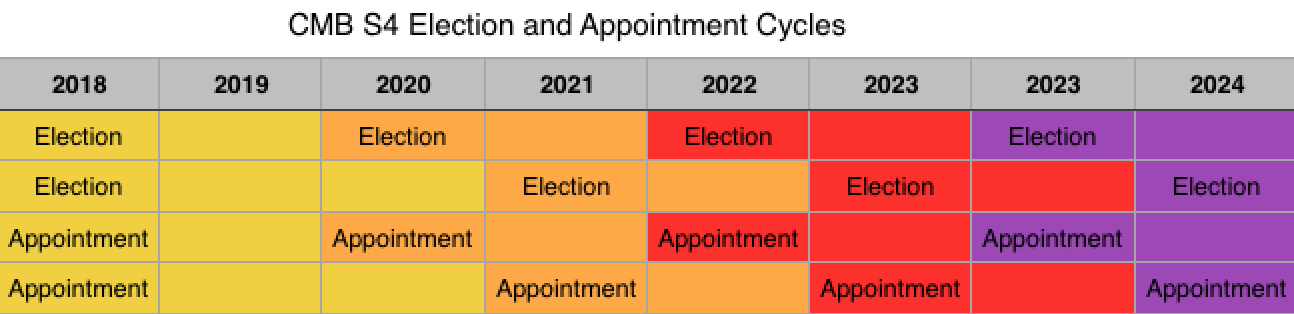
\includegraphics[width=6.5in]{Election_cycle_v2.png}
\end{center}
\caption{CMB-S4 Election and appointment cycles. For the first election, $\sim\ 50$\% of the terms are for three years rather than the nominal two, to enable staggered elections/appointments going forward.}
\label{fig:elect_cycle}
\end{figure}

\subsection{Elections of a Co-Spokesperson}

Co-Spokespersons are elected to two-year terms. All Senior Members (see \S\ref{sec:memtypes}) may  run for these positions.  %presented at the GB meeting closest to January 1 each year. 
%The Co-Spokesperson elections will occur prior to elections of the Governing board. 
%As a Co-spokesperson can not be a voting member of the GB, if 
If a Voting Member of the GB is elected as a co-Spokesperson, they must resign their GB seat prior to the start of the co-Spokesperson term and this vacancy will be filled in the next GB election. 

Prior to the election, Voting Members are asked to nominate individuals for Spokesperson to the Election and Voting Commission. Each voter may nominate one candidate and self-nominations are accepted. %A minimum of two nominations is  required for a nominee to be eligible to appear on the slate of election candidates. 
After a nomination period, the EVC will consult with the nominees to ascertain their willingness to stand for the election.
Each Voting Member votes for a single candidate for each open Spokesperson position. In the event of a tie, a runoff election will be held between the two candidates that have the same number of votes. 

%The elected candidates will take office when the EVC announces the results of the election to the Collaboration via email. 

If no candidate agrees to stand for election, the terminating co-Spokesperson will continue to serve for six months, after which a special election will be held. The term of the individual elected in a special election will be reduced by the amount needed to cause the sum of their term and the additional months served by the terminating Spokeperson to equal two years.


%The election is held through an on-line poll, with votes submitted by Voting Members. The EVC will preside over the election results. Each candidate will provide a Candidate Statement to the EVC, which will collect these documents and make them available to the Collaboration via the CMB-S4 internal web page prior to the balloting. The EVC, in consultation with the GB  determines the detailed timing of the balloting and determines procedures for dealing with any election situations not anticipated in the bylaws. Each Voting Member votes for a single candidate for each vacant position. %; in the first election, in which two Spokespersons will be selected, collaboration members may vote for two candidates. 

%The EVC checks the ballots against the list of qualified voters and tallies the votes. 
%For the first election, the two candidates with the most votes will be elected Spokesperson, with the candidate with the highest vote total selected for a three-year term to enable staggered terms for the co-Spokespersons.  
%In the event of a tie, a runoff election will be held between the two candidates that have the same number of votes. The elected candidates will take office when the EVC announces the results of the election to the Collaboration via email. 

\subsection{Council and Committee Chairs}
The co-Chairs of the Science Council, and the Chairs of the Membership Committee and the Publication and Speakers Committee are elected to two-year terms. All Senior Members (see \S\ref{sec:memtypes}) may  run for these positions.  If a Voting Member of the GB is elected to one of these positions, they must resign their GB seat prior to taking office as Chair, and this vacancy will be filled in the next GB election. 

Prior to the election, Voting Members are asked to nominate individuals for the Chair positions to the EVC.   Self-nominations are accepted.
After a nomination period, the EVC will consult with the nominees to ascertain their willingness to stand for the election. Candidates are only allowed to stand for one open position. 
Each Voting Member votes for a single candidate for each  open  Chair position. In the event of a tie, a runoff election will be held between the two candidates that have the same number of votes. 

If no candidate agrees to stand for election, the terminating Chair will continue to serve for six months, after which a special election will be held. The term of the individual elected in a special election will be reduced by the amount needed to cause the sum of their term and the additional months served by the terminating Chair to equal two years.


\subsection{Governing Board Elections }
\label{sec:gb-elections}

The 18 GB Members drawn Senior Members of the Collaboration are elected to two-year terms.  All Senior Members may  run for these positions. The one GB Member drawn from the Postdoctoral Members of the Collaboration is elected for a one-year term.

The election for the Senior Members on the GB proceeds as follows. 
Prior to the election, Voting Members are asked to nominate individuals for the GB to the EVC.   Self-nominations are accepted. After a nomination period, the EVC will consult with the nominees to ascertain their willingness to stand for the election.
Each Voting Member votes for a single candidate for each vacant GB position.  % In the event of a tie for the last open position, a runoff election will be held between the two candidates that have the same number of votes. 


%Every year, following completion of the Spokeperson election and any required \exec \ elections, the EVC then carries out elections for seats on the Governing Board whose term is expiring in less than 12 months. The EVC first solicits self-nominations for Governing Board membership and candidate information is then circulated to qualified electors as defined in the membership section of these bylaws. 
%Electors vote via email, with the votes tabulated by the EVC members not standing for election (or, in cases where the whole committee is conflicted, by a third party appointed by the Co-Spokespersons). 
%Each Voting Member may vote for up to 10 candidates, or fewer as mandated by the EVC.
% of the total number of board members. 

The election for the Postdoctoral Member of the GB follows the same procedure, with the exception that only \textcolor{red}{Postdoctoral Members are eligible to both nominate and vote for candidates for this position.} 

After the initial GB is established, it is to amend these bylaws to establish whether to have separate votes different categories of representation on the GB or to continue with a mixed election/appointed governing board model as described in Appendix~\ref{app:first_election}. It is the expectation that the GB be evolve to a fully elected body as the Collaboration matures.


%\subsubsection{The First Election of the Governing Board}
%Prior to the first election, the ICCC will define various categories of representation it deems important to include on the GB (possibly including e.g., ``tenure-track" early career scientists,  historically underrepresented groups, members from partner countries with significant membership, members of small institutions, representatives of existing CMB programs, etc). For the first election, the top 10  vote-receiving candidates are automatically selected for the GB. If representation requirements outlined above are unfulfilled by the elected candidates the remaining open seats are filled via total votes cast until seats are needed to ensure representation requirements are met. At this time the outgoing ICCC is empowered to fill the open seats to meet these requirements. 
%To enable offset elections (to ensure an element of continuity in the GB), 50\% of the first GB members will serve 3 year terms as determined by random draw. 

%\subsubsection{Election of the Governing Board after the establishment of the Collaboration}
 %After the collaboration is established, the GB is to amend these bylaws to establish whether to have separate votes for each category of representation or to continue with a mixed election/appointed governing board model. It is the expectation that the GB be moved to a fully elected body as the collaboration matures. 

\subsection{All Other Elected Positions}
For other elected Collaboration roles, the EVC is charged with establishing election rules and conducting these elections. Note that the EVC cannot make voting requirements more restrictive than those for the main body elections. Terms of elected positions are limited to durations of at most two years. 

\section{Councils and Committees}
\label{sec:councils}
Four of the organizational structures overseen by the Spokespersons have representatives on the \exec\ as described in 
\S\ref{sec:exec}.  These are the Science Council, the Technical Council, the Membership Committee and the Publications and Speakers Committee.  Their composition and charges are described in this section.  Three other standing committees for the Collaboration have been defined at this time and are described below.  

\subsection{Science Council and Analysis Working Groups}
\label{sec:SC}

\textbf{The Science Council works closely with the Spokespersons to coordinate the key scientific objectives of the Collaboration}.  The Science Council is led by two co-Chairs elected by the Voting Members of the Collaboration, who also serve as Members of the \exec.   \textcolor{red}{The Science Council chairs serve with two-year terms and are limited to two consecutive terms with one year off required before standing again.}
The remaining Members of the Science Council are the co-coordinators of the various Analysis Working Groups. These Working Groups are open to all Collaboration Members, and will be formally established by the Spokespersons.  

The Science Council approves the projects that lead to publications and is responsible for maintaining a list of Key Science topics  (\S\ref{sec:pubprop}). \textcolor{red}{It is charged to work closely with the Co-Spokespersons and the Executive Team to ensure that the key science goals of the Collaboration are achieved.} 

Each Analysis Working Group will have two co-coordinators who  serve for two-year terms with the exception of one initial coordinator who will serve for a three-year term to enable staggered appointments in the future.  The Science Council Chairs will solicit self-nominations for these co-coordinator positions. The Spokespersons will appoint coordinators with the advice of the Science Council Chairs, and will consider the distribution of early and late career Members when making these appointments. Coordinators will ordinarily not serve back-to-back terms.


\subsection{Technical Council and Technical Working Group}
The Technical Council works closely with the Spokespersons to coordinate the technical aspects needed to meet the scientific objectives of the Collaboration.  The Technical Council is led by two co-Chairs appointed by the Spokespersons.  The two Chairs serve as Members of the \exec.   The co-coordinators of the various Technical Working Groups are all Members of the TC.   These Working Groups are open to all Collaboration Members, and will be formally established by the Spokespersons.   

Each Technical Working Group will have two co-coordinators who serve for two-year terms with the exception of one initial coordinator who will serve for a three-year term to enable staggered appointments in the future, as needed.  The Technical Council Chairs will solicit self-nominations for these co-coordinator positions. The Co-spokespersons will appoint coordinators with the advice of the Technical Council Chairs, and will consider the distribution of early and late career Members when making these appointments.

We anticipate the role of and/or the need for the Technical Council will be readdressed in these Bylaws when a Project is formed.

\subsection{Membership Committee}

The Membership Committee (MC) consists of seven people including a Chair. The Chair is elected following the election cycle of the Collaboration with  two-year terms, and is limited to two consecutive terms with one year off required before standing again. \textcolor{red}{The six remaining members are appointed by the \shorte\ following approval of the slate of proposed members by the Governing Board.  These members have the same term limits as the elected chair.} If a MC Member leaves before their term is complete, the \shorte\ will appoint\textcolor{red}{---with Governing Board approval---} a replacement to finish out their term.  MC Members can be removed by a supermajority of the GB at any time.  


The appointed Members of the MC should represent the overall Collaboration, and there should be at least two Members from the Technical Working Groups and two Members from the Analysis Working Groups on the MC.  This balance may be amended as the scientific needs of the Collaboration evolve. % \Comment{This leaves two spots to encompass people who might not fall neatly into either group.}

The duties of the MC  are to review and evaluate membership applications, review annual activity reports, and recommend changes in membership status. The MC maintains an up-to-date list of all Members, available on a public website.  The MC in consultation with the \shorte\ will work with applicants and continuing Members to identify roles and infrastructure tasks that add value, avoid redundancy, and make the Collaboration as efficient as possible.  


\subsection{Publication and Speakers  Committee}
\label{sec:pubcouncil}
The Publication and Speakers Committee (PSC) consists of thirteen people including a Chair. The Chair is elected following the election cycle of the Collaboration with  two-year terms, and is limited to two consecutive terms with one year off required before standing again. There are two sub-committees which together comprise the PSC: the Publications Board with eight Collaboration Members and the Speakers Bureau with four Collaboration Members. \textcolor{red}{The Chair of the PSC chairs both of the subcommittees.} \textcolor{red}{The twelve non-elected committee members are appointed by the \shorte\ following approval of the slate of proposed members by the Governing Board.} The twelve appointed members serve with the same term limits as the elected Chair.  Roughly half of each group should be pre-tenure. If a PSC Member leaves before their term is complete, the \shorte\ will appoint\textcolor{red}{---with Governing Board Approval---}a replacement to finish out their term.  PSC members can be removed by a supermajority of the GB at any time.  
 




\subsection{Junior Scientist Advancement Committee}

The role of the Junior Scientist Advancement Committee (JSAC) is to ensure that junior members (defined as students and postdoctoral researchers) within the Collaboration are represented, assisted, and supported throughout the  tenure of the Collaboration. This will include arranging mentors for junior members who desire mentorship, and facilitating junior member career advancement through relevant workshops and other activities. The JSAC Chair and deputy Chair are appointed by the \shorte\ after the elections and serve 2 year terms that parallel the Collaboration's elections. Membership on the JSAC is open to volunteers from the Collaboration, with the approval of the JSAC Chair. 


\subsection{External Collaborators Committee}

The role of the External Collaborators Committee (ECC) is to provide the necessary link to external follow-up observations or survey data that required to maximize the science return from CMB-S4. The ECC Chair and deputy Chair are appointed by the \shorte\ after the elections and serve terms that parallel those of the elected Collaboration positions. The Chair will appoint additional members as required to ensure adequate knowledge of the collaborations being pursued resides in the ECC. Self nominations for consideration of ECC are expected. 

The committee will draft all the necessary documents for external collaboration agreements and memorandums of understanding (MOUs). These will be presented to the Spokespersons and the  \shorte who have the ability to amend and alter these agreements and MOUs as they choose. Such agreements are then brought forward by the Spokespersons to the GB for final approval. %\Comment{This might also fall under Project management.}

\subsection{Education and Outreach Committee}

The Education and Public Outreach (EPO) Committee is responsible for initiating, overseeing, and recording the Collaboration's efforts in the areas of public outreach and education. Its mission is to disseminate Collaboration results to the public and increase general scientific literacy. The committee is overseen by the \exec \ and members are appointed by the \shorte after solicitation of nominations from the full Collaboration. The Chair is appointed by the Spokespersons. Terms on the EPO Committee are for two years, with some initial three-year terms to allow staggered appointments.   A presentation of EPO efforts and written documentation of activities must be provided to the \shorte at each Collaboration meeting or when requested by the \shorte. 

\section{Membership Policy}

The Collaboration consists of Ph.D. scientists, engineers, Ph.D. thesis students %undergraduate students, 
and others who contribute significantly to the CMB-S4 program. Membership conveys certain rights as described below, but comes with the obligation of an ongoing commitment of a substantial fraction of members' research time to the CMB-S4 program.

\vspace{0.2in}
\noindent


%\subsection{Membership Committee}
%The duties of the Membership Committee are to review and evaluate membership applications, review annual activity reports, and recommend changes in membership status. 

\subsection{Membership Types}
\label{sec:memtypes}
Five types of members are defined here.  
\begin{itemize}

\item {\bf Senior Member:} A Senior Member of the Collaboration is a member who has a permanent appointment or an appointment, that under normal circumstances can be expected to be renewed indefinitely.   This includes tenure-track appointments at universities and their equivalents elsewhere.  

\item {\bf Postdoctoral Member:} A postdoc working with a Senior Member at their institution can be designated as a Postdoctoral Member by that Senior Member.  Postdocs that reside at an institution where there is no Senior Member can apply to become a Postdoctoral Member and have their application evaluated by the Membership Committee on a case-by-case basis. 

\item {\bf Student Member:} A graduate student working with a Senior Member at their institution can be designated as a Student Member by that Senior Member.  We do not anticipate granting membership to students who are not supervised by a Senior Member.

\item {\bf Provisional Member:}  A provisional member is a someone who has not yet been approved for regular
(Senior, Postdoctoral or Student) member status.  This status applies to all new Student and Postdoctoral members
(including, for example, in an existing Senior Member's group).  It also applies to potential Senior Members whose membership
application has been approved.  This is intended to be a temporary status, typically a year, allowing the member to demonstrate
sufficient constructive engagement with the Collaboration.

\textcolor{red}{
\item {\bf Legacy Member:}  A Legacy Member is a former member who contributed in a key manner to the Project or analysis infrastructure, but is no longer engaged with the Collaboration and is therefore no longer a member.  This status is intended to convey authorship rights to such former members, and to bypass the normal membership procedures should they wish to re-engage with the Collaboration.
}

\end{itemize}



\subsection{Membership Rights}\label{sec:memberrights}

Herein, ``Members'' refers to Senior, Postdoctoral, Student and Provisional Members (but not Legacy Members) unless otherwise qualified.  

\begin{itemize}

\item Senior and Postdoctoral Members are Voting Members.  Voting Members  have the right to vote to ratify Bylaws and amendments to Bylaws, and vote in elections for Spokespersons, Governance Board representatives, and the elected positions including the Chairs of the Science Council, and the Membership and Publication and Speakers Committees.  %vote for representation on the Governing Board.  

\item Members have full data access, including during the proprietary period for data that are eventually released.

\item Members (including Legacy Members) have the right to be listed as a co-author on CMB-S4 publications as specified in the Publication Policy.

\item Members have access to computational resources designated for CMB-S4, according to the policies of the relevant Computational Resources Working Group.

\end{itemize}

\subsection{Membership Requirements}

 Members must commit effort to approved infrastructure tasks.   
The Membership Committee will work with the \exec\ to define and recommend infrastructure tasks that need filling, 
\textcolor{blue}{ and to define and communicate with members the level of expected effort.}
Tasks can include,  for example, designing, building, and testing software, hardware, or simulations; contributing to commissioning and observations; and management tasks. 
Just as for the hardware, we anticipate having a collaboration-wide architecture for the software.  Thus, members will be expected to comply with interface, documentation and code review requirements in support of the goals of the Collaboration.   Other ways of contributing include taking on roles in the governance, including membership on the GB, EVC, ET, or the Councils and Committees described in \S\ref{sec:councils}.




\subsection{Membership Application and Approval Process}
After the Collaboration is formed with a first set of initial members (see \S\ref{sec:initmembership}), the process for membership to CMB-S4 will be as specified below.

\begin{itemize}

\item Potential Senior Members will apply for Provisonal Membership via a written application where they specify their proposed work on CMB-S4. 

\item Independent postdocs not co-located with a Senior Member can apply for Postdoctoral Membership and have their application reviewed on a case-by-case basis. 

\item Postdoctoral members can apply for ``Intended Senior Membership Status", which would convey that the postdoc will have Senior Membership status when preparing to move to a specified permanent appointment or an appointment that, under normal circumstances, can be expected to be renewed indefinitely.  The Membership Committee will decide the requirements for achieving this status, the achievement of which grants Senior Membership at the new institution.

\item Applications are reviewed by the Membership Committee. The Membership Committee recommends membership to the Governing Board.  The Governing Board approves membership.

\end{itemize}

\subsection{Initial Membership}
\label{sec:initmembership}
The Collaboration will initially consist of members that were eligible to vote on these governance bylaws (by virtue of attendance at two or more Collaboration meetings, or a successful petition for eligibility), and cast a vote on them. 

%The Collaboration will initially consist of members who have satisfied the following criteria:
%
%\begin{itemize}
%\item Attended at least two Collaboration meetings, and 
%
%\item Voted on the governance bylaws.
%\end{itemize}

Within the first year of the Collaboration's establishment, prospective members can be granted membership by successfully petitioning the Membership Committee despite not satisfying the above criteria.  The Membership Committee may approve such applications during the first year without action by the Governing Board.  

The Collaboration will initially consist of members that were eligible to vote on these governance bylaws (by virtue of attendance at two or more Collaboration meetings, or a successful petition for eligibility), and cast a vote on them. 

\subsection{Membership Review and Changes in Status}
The membership status of each member will be reviewed by the Membership Committee each year. 

\begin{itemize} 

\item Each Senior Member, and each independent postdoc not co-located with a Senior Member, will submit an annual activity report to the Membership Committee.  Reports of the Senior Members should include discussion of the activities of their supervisees (e.g., postdocs and students) in their report. The Membership Committee will review those reports, consulting with Collaboration members and Working Group leaders as appropriate.

\item Provisional Members will submit a annual activity report to the Membership Committee, which will review the report and determine whether the Provisional Member should be promoted to a Senior Member status, continue as a Provisional Member, or have their membership revoked.  Provisional Membership is intended to be a temporary status.

\item Members leaving the Collaboration may be granted Legacy Membership upon review by the Membership Committee and approval by the GB.

\item If the effort of any member over the previous year seems lacking, the Membership Committee will bring this to the attention of the Spokepersons and the GB.  This can also be done at any time, should the Membership Committee deem the actions of a member to have been egregious and detrimental to CMB-S4.

\item The Governing Board has the authority to grant or terminate all forms of membership.

\item When a person's membership in the Collaboration ends, they will no longer have access to the CMB-S4 document and database repository, internal forums, computing resources and data.  Authorship rights will continue, or not, as prescribed in the Publication Policy bylaws.


\end{itemize}

%\subsection{Procedure to Change Membership Policies}

%The Governing Board may change Membership policies by a 2/3 majority vote of voting members.

%\section{Collaboration and Institution Membership}

\subsection{Requirements for Admission}

The CMB-S4 collaboration consists of Ph.D.\ scientists, engineers, Ph.D. thesis students, undergraduate students, and others who contribute significantly to the CMB-S4 program. A rough guideline is that all collaborators should devote a substantial fraction of their research time to the CMB-S4 program over a period of several years.
Visiting scientists and engineers (henceforth visitors), such as faculty members on sabbatical at a CMB- S4-affiliated institution, may also be admitted to the collaboration as short-term members, provided they devote a substantial portion of their research time to the collaboration.

The process of admission to the collaboration shall accord with the membership rules applicable to their degree of seniority. A senior member of the collaboration is a member from a collaborating institution who has a permanent appointment or an appointment that under normal circumstances can be expected to be renewed indefinitely. All other members of the collaboration are regular members. Senior members are admitted to the collaboration individually. Regular members are selected by their institutions. The only distinction between senior and regular members is the method by which they are admitted to the collaboration.
Senior members are admitted to the collaboration in one of four ways:
\begin{enumerate}
\item by being on the qualified elector list at the time of the initial spokesperson election,
\item by being on the approved list of senior members when their institution was admitted to the collaboration,
\item by being a regular member of the collaboration and receiving a position at any collaborating institution that would qualify him or her for senior membership status,
and
\item by individual application.
\end{enumerate}
A senior physicist at a collaborating institution who is not a member of the collaboration, and who wishes to join the collaboration, applies for membership in the same way as a new institution, as provided in Section 6. This procedure applies as well to visiting senior personnel applying for short-term membership.

The membership list is distinct from the author list described in Section \ref{sec:pub}.

\section{Admitting New Institutions}

To apply for membership in the CMB-S4 collaboration, representatives from the institution should first confer with the spokesperson. The representatives then submit a written proposal to the IB chair at least two weeks prior to the meeting of the IB at a regularly scheduled collaboration meeting. The IB chair circulates the proposal to IB members prior to the meeting and puts consideration of the application on the meeting agenda.

The proposal should describe the contributions that the prospective institution proposes to make to the collaboration and should include a list of the proposed senior members from the institution. The spokesperson will present the proposal to the collaboration by the prospective institution. This presentation should occur prior to the IB meeting held during the same collaboration meeting. The IB may: (1) approve the proposal and formally admit the institution to the collaboration at that meeting, (2) request further written clarifications to be considered at the next collaboration meeting, or (3) reject the proposal. The IB will attempt to make decisions on admission of new institutions by consensus. If consensus is not possible, a vote by secret ballot will be taken on admission. Admission will require a favorable vote by a super-majority of IB members present and voting.

\section{Removal of Collaborators and Institutions, Updating Membership and Leaving an Institution}

\subsection{Removal of Collaborators and Institutions}

Annually the IB Chair, in consultation with the spokesperson, will identify inactive institutions, using the criterion that an active institution has performed a reasonable amount of work on CMB-S4 within the previous twelve months. The IB may remove inactive institutions from the collaboration by a super- majority vote.

Individual collaborators who have not performed a reasonable amount of work on CMB-S4 for a period of at least twelve months, or whose behavior has been egregious and detrimental to CMB-S4, may be removed from the collaboration at an IB meeting by a super-majority vote of the IB members present and voting.

\subsection{Updating CMB-S4 Membership Rolls}

Each CMB-S4 IB member will be responsible for updating and verifying the collaboration membership list for his/her institution. A yearly questionnaire will be distributed by the IB chair to each institution to help keep track of all members and their status.

\subsection{Leaving a Collaborating Institution}

Individuals maintain their membership in the collaboration automatically for one year after they leave any collaborating institution. They can maintain a longer-term association with CMB-S4 by being ``adopted'' by a collaborating institution, with this process being approved by the IB on a case-by-case basis.

When a person's membership in the collaboration is terminated, they will no longer have access to the CMB-S4 document and database repository, internal forums, computing resources and data.





%\section{Publication and Speakers Council}
\label{sec:pub}

%test message
%\textcolor{red}{To be filled in by Publications WG}. 

%\Comment{\textbf{Formal Publication and Speakers Bureau Policy - 2nd draft.}  The policy below is a draft formal bylaws.  It is not a consensus document of the Interim Publications Working Group.  It is meant to be a complete, self-consistent policy to spur discussion and gather thoughts and suggestions about how the pieces need to work together.  The policy attempts to lay out the various responsibilities of publication board and speakers bureau members, working group coordinators, as well as relationships to other parts of the collaboration structure, like the governing board  and membership committee. These responsibilities could be redistributed in different ways. What projects/paper are ``Key," and get alphabetical author lists, if we adopt that model, is a point of contention, and we fill seek further input from the collaboration. We consider several possibilities for Key topics at the very end.}


%CMB-S4 publication and talks bylaws Established March 2018

\subsection{Principles}
This policy seeks to ensure an equitable distribution of credit for work in the CMB-S4 Collaboration, to encourage and incentivize active work by collaboration members, and to ensure the resulting publications are of high quality. The authorship policy of the American Physical Society (2002) states: \textit{``Authorship should be limited to those who have made a significant contribution to the concept, design, execution or interpretation of the research study. All those who have made significant contributions should be offered the opportunity to be listed as authors.''}\footnote{\url{https://www.aps.org/policy/statements/02_2.cfm}}

The Publication Policy will apply to all projects and publications that employ collaboration resources, including unreleased data, simulation codes and products, hardware and software
engineering designs, and analysis pipelines. All CMB-S4 collaboration members agree to the publication policy upon joining, and if they leave the collaboration, they are bound by it for two years afterward.

\subsection{Organization}
The execution of the policy shall be overseen by a Publication and Speakers Council chaired by an elected representative from the Executive Team.  There are two sub-committees: the Publications Board with eight collaboration members and the Speakers Bureau with four collaboration members. Roughly half of each group should be pre-tenure. The Spokespersons and Executive Team shall appoint members to these positions for staggered two-year, non-consecutive terms. The collaboration Spokespersons will also help to navigate and resolve potential conflicts. The Science Council approves the projects that lead to publications. The Membership Board will keep track of active collaboration members and legacy member for the purposes of establishing author lists for papers.

\subsection{Project Proposal Process}

%\Comment{[Ed. note: The entire concept of ``Key Science'' papers is up for discussion, but only bits are highlighted below to avoid making the whole paragraph red.  Such a concept (under various names) is employed is many collaborations.  At the very end, we place possible suggestions for ``Key" topics.]}

Any collaboration member may propose a collaboration research project to an appropriate Science or Technical Working Group.  Such a project is work that is intended to result in a journal publication after a fixed term, or a small set of related publications.  There are three categories for projects:
\begin{enumerate}
  \item Projects that are designated as ``Key Projects'' represent the main science goals of the CMB-S4 collaboration (or forecasts for what we will achieve), where the collaboration must speak with a single voice.  
\item ``Standard'' analysis projects represent other science goals and use collaboration science data.  
\item Other forecasts and technical reports are collaboration-vetted projects that do not require collaboration science data and may lead to a publication or conference proceeding.  
\end{enumerate}
The Science Council will maintain the list of Key Science topics, to be established prior to any projects being initiated.  Topics can be added to the Key Science paper list and reviewed in coordination with the Publication Board.

The Publication Board will establish the template for project submission.  The project proposal document will designate a project leader and team, and describe the project, its estimated completion date, and final products.  Work on collaboration data should apply toward a collaboration project: failure to submit a project at its initiation, or writing a paper on internal collaboration data for submission when the data become public, will be considered a violation of the policy.  The same general type of analysis on subsequent observing seasons or data releases will be considered separate projects.

After discussion, resolution of conflicts, and consensus within the Working Group, the Working Group Coordinators will submit the project to the Science Council with a project category recommendation as a Key project, standard project, or theory forecast / technical report.  At this time the working group coordinators will announce the proposal to the Collaboration for a two-week consideration period, for discussion and further resolution of conflicts.  Addressing overlap between projects may require revision of the proposed project, and will be negotiated by the Working Group coordinators, Project Leaders, and Spokesperson(s).  Teams should welcome to join any colleagues that wish to make a defined and useful contribution to the project.

The Science Council may then approve the project or send it back to the Working Group for further revision.  In the event of a tie vote in the Science Council, the collaboration spokesperson  will cast the deciding vote.  When approved, the Publication Board will record the proposal in its project database.  Once recorded, the collaboration may not re-classify a standard project as key without the written agreement of all named project team members.  If there is any substantial change in the scope of a project as it matures, the Project Leader should adjust the project description accordingly, which will result in a new announcement and opportunity for collaboration review.

Projects led by thesis students will be given special consideration to protect them from competition within the collaboration.  Projects that require joint work with an external collaboration will require a memorandum of understanding set up by the External Collaborators Committee that specifies authorship and publication policies for that work.  These should be as compatible as possible with the respective collaboration policies.  Projects may add individual external collaborators to the team provided that no unreleased data is provided to them.

Project teams have the responsibility to carry projects to completion and publication.  The Publication Board will query the working group coordinators twice yearly for progress reports on all projects, and forward the results to the Science Council.  Any projects without progress for one year will be noted as ``inactive'' and will be dropped from the database if there is still no progress at the next review.

\subsection{Authorship}
%\Comment{[Ed. note: Aside from the concept of ``Key science'' vs ``standard papers,'' the main dispute in this section relates to opt-in/opt-out as the default, or whether a weak opt-in is any better than an opt-out.]}

For the purposes of authorship, ``active members'' consist of Senior, Postdoctoral, and Graduate members of the collaboration as defined in the membership council bylaws.  Provisional member may appear on papers to which they actively contribute.  The three types of projects differ in their authorship rules.

\begin{enumerate}
\item For Key papers, all active members of the collaboration and all legacy members will automatically be placed on the author list.  The author list will start with ``The CMB-S4 Collaboration'' and otherwise be alphabetical.  The project team will designate a small number of corresponding authors to signify those most involved with the work.  The Membership Board will provide the current list of eligible active and legacy members to the Publication Board, who will maintain an online process for members who choose to opt out of the paper.
\item For standard papers, the author list will be two-tiered.
%  The first tier will typically consist of untenured (or equivalent) members of the project team, ordered according to their preference.  (The publication panel can allow exceptions for senior scientists in the first tier in rare cases when justified by their contribution.)
  Project teams may organize the first author tier as appropriate for the paper, and although not required, conventionally the tenured members of the project team will appear in the second, alphabetical tier of authors.
  %The project leader will typically be the first author.
  The second tier will consist of all active members and legacy members that choose to opt in online after an email notification.  The final line of the author list will be ``The CMB-S4 Collaboration.''
  \item For other forecasts and technical reports, the author list will consist of the project team only, plus any collaboration members that contributed to the study, as determined by the project team and appropriate working group coordinators, unless those author opt out.  The author list should be ordered according to the preference of the project team, followed by ``for the CMB-S4 Collaboration.''  For conference proceedings, the author list may be the single person who presented.
\end{enumerate}


Any disputes regarding authorship will be resolved by the Publication Board with the Spokespersons providing  tie-breaking votes if necessary.  If an eligible member is unable to opt in, due to an unforeseen circumstance, the Publication Board may add them to the author list.

\subsection{Collaboration Review and Paper Submission Process}
%\Comment{[Ed. note: the timing of the formation of the review team with respect to collaboration-wide review is a point of debate.  Some feel that the reviewers should be assigned early, so that they can iterate more with the authors on the paper.  Others feel the assignment of the editors should only happen at the beginning of the collaboration-wide formal review, otherwise the review process is too closed and not democratic.  The scheme below has a mix of these features.]}
 
The project leader and the project team have the responsibility to draft the publication based on their research.  All collaboration papers will have a title following the template, ``CMB-S4: \textit{results of amazing research}.''  These papers will be developed in coordination with the relevant working groups, and kept in a repository that is visible to the whole collaboration.  Any collaboration member may comment on the project at any time.  When the paper matures to an advanced draft, the working group coordinators will request that the Publication Board form an internal review committee.  

This internal review committee consists of a primary and a secondary reviewer who have the responsibility that the collaboration's publications are of uniform and high quality.  The reviewers are not current members of the Publication Board, but the Publication Board assigns one of its members to oversee the review of the paper as a rapporteur.  At least one of the reviewers or rapporteur should be a senior scientist who can insulate junior participants (whether authors, reviewers, or rapporteurs) from unfair criticism, if it occurs.

The Publication Board will notify the full collaboration that the internal review committee has formed.  Collaboration members may comment on the draft at any time, but when the authors are ready, the Publication board will send an announcement of a formal three-week comment period.  After the this comment period, the reviewers will provide a written report on the paper to the authors and Publication Board.

All public comments, from collaboration members and from reviewers, are to be posted to a centralized location maintained by the Publication Board, along with the authors' responses.  All collaboration members have access to these previously asked questions and responses.

The working group coordinators and rapporteur oversee iterations on the draft.  When the reviewers, working group coordinators, and rapporteur are satisfied that comments have been appropriately addressed, they present the paper to the Publication Board, who gives final permission and sets the date for paper submission.  The submission date is announced to the collaboration with a notice for final reading.  

In total, all projects/papers will have four formal public announcements to the collaboration:
%\begin{enumerate}
%\item when proposed,
%\item when the review committee forms,
%\item when the formal comment period begins, and
%\item when the call goes out for final reading before submission.
%\end{enumerate}
(1) when proposed,
(2) when the review committee forms,
(3) when the formal comment period begins, and
(4) when the call goes out for final reading before submission.
  Projects will also naturally be discussed in plenary teleconference calls, progress reviews, and working group reports.

All CMB-S4 publications, including proceedings and theses, must include a standard acknowledgment, agreed to and updated by the Governing Board, and made available by the Publication Board.  The CMB-S4 Collaboration will pay the page charges for Key papers. For all other papers, the page charges are the responsibility of the authors.

Any disputes regarding the review process will be resolved by the Publication Board with the Spokespersons providing tie-breaking votes if necessary. In the case of a time-sensitive discovery, the review period may be shortened by unanimous consent of the Publication Board.

Graduate thesis and dissertation documents are exempted from collaboration review, but related publications (e.g.~developed from an individual chapter) are subject to review.

\subsection{Talks and Public communications}
%\Comment{[Ed. note: This is based on the non-controversial interim policy.]}

The role of the Speakers Bureau is to help collaboration members give more and better talks in support of the CMB-S4 collaboration. The duties of the Speakers Bureau are to:
\begin{itemize}
\item Solicit invitations to conferences and identify good venues for contributed talks.
\item Actively solicit speakers for invitations or notable conferences with no volunteer speakers. Priority and consideration should be given to the teams from projects where alphabetical author lists may obscure their role. 
\item Promptly respond to requests for speakers from conference organizers and act a point-of-contact for people who want some CMB-S4 speaker but do not have specific ideas.
\item Curate a library of standard plots and slides for speakers to use in talks.
\item Maintain a library of past CMB-S4 talks.
\item Address overlap from multiple requests to give talks on the same subject at the same conference, ideally by suggesting focus changes to make them on different topics. Talk prioritization will be at the committee's best judgment, but should reflect contributions to the topic in question, career status, whether the speaker was invited, and other similar factors.
\end{itemize}

To give a talk, whether contributed to a conference/workshop or invited,  a collaboration member must notify the Speakers Bureau. This ensures that the Speakers Bureau has a chance to address overlapping talk request or, in the case of declined invitations, can locate another appropriate speaker.  The talks policy applies to all workshops, meetings, colloquia, public lectures, and seminars.  The policy does not apply to talks on other subjects that contain brief advertisements for CMB-S4, to invited presentations that must remain confidential for programmatic reasons (e.g.~certain agency reviews or presentations to private foundations or donors), or to informal presentation at collaboration members' home institutions.  

All talks must maintain confidentiality for the project. For all talks except those exempted in above, collaboration members must send abstracts and titles to the collaboration at least three days prior to submission, or as soon as possible in the event of last-minute invitations. Slides must be sent to the collaboration at least one week before being presented and should include ``for the CMB-S4 collaboration" on the title slide.

Unpublished results shown in talks, including those talks exempted in above but not including thesis defenses, must be approved for public release by the collaboration before being shown. Such results should be marked ``CMB-S4 PRELIMINARY" on slides until publication.  Final public oral presentations for thesis student are not bound by the speakers policy and may show unreleased data, but must maintain confidentiality of major results.

The Speakers Bureau will maintain records of all presentations given in the name of the collaboration, and serve as a clearinghouse for talk invitations forwarded from any member.  

\subsection{Violations of the Policy and Remedies}
Violations of the policy will be addressed by the Publication Board, which will forward violations and recommend a remedy to the Executive Team.  Minor infractions will receive a warning, while repeated or severe infractions may warrant suspension from project teams or working group activities, removal from such groups, or expulsion from the collaboration as determined by the Governance Board.

%\subsection{Amendments}
%Any collaboration member can propose an amendment to the Publication/Speakers Policy. The Publication and Speakers will jointly discuss the amendment and forward a recommendation to the Governance Board for a final, majority vote.










%\subsection{Scope}
%The authorship policy spells out the criteria and procedures for determining which members of the collaboration will be listed as authors on publications. The author list will be comprised primarily of currently active members of the collaboration that satisfy the effort and shift criteria discussed below. Former members of the collaboration that have recently left can also opt to be included as legacy authors. Procedures for adding special cases and for addressing appeals are also specified. The formulation of the author list is treated separately for physics papers and technical papers. In general, the author list for a given paper is considered frozen once the paper has been submitted. Exceptions to this are discussed in Section~\ref{sec:except}.


%\subsection{Current Authors}
%Current authors are scientists at the level of graduate student or above who are members of the CMB- S4 collaboration and are actively engaged in the collaboration. This includes visitors. They will have contributed a significant fraction of their research time to the collaboration in the twelve months prior to preparation of the author list.

%The initial set of proposed authors will be submitted to the IB by each of the IB representatives, who will prepare a list of proposed names at their institution, along with a brief description of their contributions and level-of-effort. The IB chair will circulate this initial list to the IB one month in advance of the vote. IB members who want a specific candidate discussed will submit the name of the candidate to the IB chair no less than two weeks before the vote, with any questions or issues, and that name will be flagged for discussion.

%The IB chair will send the names, questions and issues regarding these candidates to all IB representatives promptly. At the initial vote, candidates who have not been flagged can be accepted by acclamation; flagged names will be discussed individually with the IB representative making the case for the candidate. A majority vote of voting members will suffice to include the candidate. This group will form the default author list for all qualifying CMB-S4 publications as defined in Section~\ref{sec:pubdef}. Individual authors can opt out of being included as an author for a given publication by notifying the spokesperson.

%The current author list will be updated through this mechanism as appropriate but at least once per year, with the IB chair supervising the update. For the updates, the IB representatives will flag any new additions to the author list. Once formed, the current author list will be made available to the collaboration. Any individual member of the collaboration can petition the chair of the IB for inclusion if they believe to have been improperly excluded.

%\subsection{Voting Rules}

%A majority vote of those voting is required, and all authorship votes follow this rule unless otherwise noted.

%\subsection{Definition of Qualifying Publications}

%The current author list shall be attached to any publication, as defined in Section~\ref{sec:pubdef}, discussing a physics result, as defined in Section~\ref{sec:pubdef}. In addition, when allowed, it shall also be attached to conference proceedings.

%\subsection{Legacy Authors}
%Legacy authors are individuals who have ceased active participation in the collaboration preceding submission of a publication but choose to opt-in to the author list via email to the spokesperson. The opt-in can either be a blanket opt-in, whereby the individual?s name is automatically included in the author list for all papers, or a case-by-case opt-in, whereby the individual must contact the spokesperson for each submitted paper. An individual can exercise his or her opt-in option until their legacy period has expired. For deceased members, the blanket opt-in option will be assumed. The legacy period, which applies to visitors as well, will be set to either one year or one-quarter of the time since the person has joined the collaboration, whichever is longer. The time a person joined shall be taken from the collaboration list as maintained by the IB chair. Once the legacy period has expired the Special Author rules apply.

%\subsection{Special Authors}
%Special authors are defined as authors who do not qualify as current or legacy authors but are listed on an individual paper based on specific contributions to that paper. Engineering staff, technicians, undergraduates, and other non-physicists who have made exceptional contributions are examples of special authors, as well as scientists who have made significant contributions to the specific paper. They must be nominated for inclusion on the author list by a member of the IB.

%Visitors, whose contact with the collaboration may encompass a period of less than one year, may be accepted as authors on papers concerning topics to which they have made significant contributions, subject to the legacy period and the approval of the IB.

%For the first paper reporting, CMB-S4 individuals can either be nominated by a member of the IB, or can petition the IB chair for inclusion on the author list. In either case, both of the following conditions must be met: (1) the individual must have worked on the collaboration for at least one FTE year, and (2) the individual must have made an intellectual contribution to the collaboration. The IB must approve special author nominations and petitions by a majority vote.

%\subsection{Technical Publication Authors}

%Publications that discuss technical results, as defined in Section~\ref{sec:pubdef}, will not be required to carry the current author list. Publications in NIM, IEEE, SPIE on hardware, or specialized simulations are typical examples. The primary proponents of technical papers will create a custom author list that does not require approval of the collaboration. However, the draft manuscript must be submitted to the Publications Board (cf. Section~\ref{sec:pubdef}) and the author list to the IB. IB representatives can ask the proponents to add individuals they think ought be included on the author list.

%\subsection{Examples of Contributions Qualifying for Authorship}

%The following list gives examples of contributions; it is meant to be indicative, not exclusive, and to serve as a guideline:
%\begin{itemize}
%\item governance of the collaboration
%\item construction of the experiment
%\item maintenance or operation of the experiment ? scientific effort during the project phase
%\item simulation or data reconstruction work
%\end{itemize}


\section{Publication and Speakers Policy}
\label{sec:pub}
\subsection{Principles}
This policy seeks to ensure an equitable distribution of credit for work in the CMB-S4 Collaboration, to encourage and incentivize active work by Collaboration members, and to ensure the resulting publications are of high quality. The authorship policy of the American Physical Society (2002) states: \textit{``Authorship should be limited to those who have made a significant contribution to the concept, design, execution or interpretation of the research study. All those who have made significant contributions should be offered the opportunity to be listed as authors.''}\footnote{\url{https://www.aps.org/policy/statements/02_2.cfm}}

The Publication Policy will apply to all projects and publications that employ Collaboration resources, including unreleased data, simulation codes and products, hardware and software
engineering designs, and analysis pipelines. All Collaboration members agree to the publication policy upon joining, and to be bound by it for two years after leaving the Collaboration.
%All Collaboration members agree to the publication policy upon joining, and if they leave the Collaboration, they are bound by it for two years afterward.

{\color{red} 
The Publication and Speakers Committee will continue to refine the policy, and present a revision one year after the establishment of the collaboration for ratification by the voting members.
}

\subsection{Organization}
The execution of the policy shall be overseen by the Publication and Speakers Committee and its sub-committees (\S\ref{sec:pubcouncil}). 
{\color{red} The Science Council approves all projects that lead to publications.  The Science Council in addition establishes the slate of projects that advance the Collaboration's key science goals and it solicits the Working Groups for detailed proposals for carrying out these projects.  This is done in consultation with the ET and in accordance with the Spokepersons' yearly plan.}
The Spokespersons will help to navigate and resolve potential conflicts.
The Membership Committee will keep track of active Collaboration members and Legacy Members for the purposes of establishing author lists for papers.

%The execution of the policy shall be overseen by a Publication and Speakers Committee.  There are two sub-committees: the Publications Board with eight Collaboration members and the Speakers Bureau with four Collaboration members. Roughly half of each group should be pre-tenure. The Spokespersons and Executive Team shall appoint members to these positions for staggered two-year, non-consecutive terms. The Collaboration Spokespersons will also help to navigate and resolve potential conflicts. The Science Council approves the projects that lead to publications. The Membership Committee will keep track of active Collaboration members and legacy member for the purposes of establishing author lists for papers.

\subsection{Project Proposal Process}
\label{sec:pubprop}

%\Comment{[Ed. note: The entire concept of ``Key Science'' papers is up for discussion, but only bits are highlighted below to avoid making the whole paragraph red.  Such a concept (under various names) is employed is many collaborations.  At the very end, we place possible suggestions for ``Key" topics.]}

Any Collaboration member may propose a Collaboration research project to an appropriate Analysis Working Group or Technical Working Group.  Such a project is work that is intended to result in a journal publication after a fixed term, or a small set of related publications.  There are three categories for projects:
\begin{enumerate}
  \item Projects that are designated as ``Key Projects'' represent the main science goals of the Collaboration (or forecasts for what we will achieve), where the Collaboration must speak with a single voice.  
\item ``Non-key''  analysis projects represent other science goals and use Collaboration science data.  
\item Other forecasts and technical reports are Collaboration-vetted projects that do not require Collaboration science data and may lead to a publication or conference proceeding.  
\end{enumerate}
The Science Council will maintain the list of Key Science topics, to be established prior to any projects being initiated.  Topics can be added to the Key Science paper list and reviewed in coordination with the Publication Board.

The Publication Board will establish the template for project submission.  The project proposal document will designate a project leader and team, and describe the project, its estimated completion date, and final products.  
Projects led by thesis students will be given special consideration to protect them from competition within the Collaboration.  Projects that require joint work with an external collaboration will require a memorandum of understanding set up by the External Collaborators Committee that specifies authorship and publication policies for that work.  These should be as compatible as possible with the respective Collaboration policies.  Provisional Members and individual external collaborators may be suggested as team members.  The External Collaborators Committee must be consulted in the latter case, to determine if MOUs are required.  


Work on Collaboration data should apply toward a Collaboration project: failure to submit a project at its initiation, or writing a paper on internal Collaboration data for submission when the data become public, will be considered a violation of the policy.  The same general type of analysis on subsequent observing seasons or data releases will be considered separate projects.

After discussion, resolution of conflicts, and consensus within the Working Group, the Working Group coordinators will submit the project to the Science Council with a project category recommendation as a Key Project, non-key project, or theory forecast / technical report.  At this time the Working Group coordinators will announce the proposal to the Collaboration for a two-week consideration period, for discussion and further resolution of conflicts.  Addressing overlap among projects may require revision of the proposed project, and will be negotiated by the Working Group coordinators, publication-project leaders, and Spokespersons.  Any Collaboration Members that wish to make defined and useful contributions to the project are welcome to join the team.  Disputes will be settled by the Working Group coordinators and Spokespersons as needed.  

The Science Council may then approve the project or send it back to the Working Group for further revision.  In the event of a tie vote in the Science Council, the project is sent back.  When approved, the Publication Board will record the proposal in its project database, including its project category.  If there is any substantial change in the scope of a project as it matures, the Project Leader should adjust the project description accordingly, which will result in a new announcement and opportunity for Collaboration review.  After the definition of a project, its category can be reclassified only by unanimous written agreement of the project team and a supermajority vote of the Publication Board,  or by a supermajority vote of the GB.

Project teams have the responsibility to carry projects to completion and publication.  The Publication Board will query the Working Group coordinators twice yearly for progress reports on all projects, and forward the results to the Science Council.  Any projects without progress for one year will be noted as ``inactive'' and will be dropped from the database if there is still no progress at the next review.

\subsection{Authorship}
%\Comment{[Ed. note: Aside from the concept of ``Key science'' vs ``standard papers,'' the main dispute in this section relates to opt-in/opt-out as the default, or whether a weak opt-in is any better than an opt-out.]}

For the purposes of authorship, ``Active Members'' consist of Senior, Postdoctoral, and Student Members of the Collaboration as defined in \S\ref{sec:memtypes}.  Provisional Members and external collaborators may appear as authors on papers when they are part of the project team.


\begin{enumerate}
\item For Key Project papers, all Active Members of the Collaboration and all Legacy Members will automatically be placed on the author list.  The author list will start with ``The CMB-S4 Collaboration'' and otherwise be alphabetical, unless the Publication Board agrees that the paper should be submitted to a journal which requires the first author to be an individual.  In that case, the author list will be alphabetical.
  {\color{red}\sout{The project team will designate a small number of corresponding authors to signify those most involved with the work.}}
  The Membership Board will provide the current list of eligible Active and Legacy Members to the Publication Board.
  {\color{red}
    \sout{Anyone who chooses to opt out of authorship for a given Key Project paper must  notify the Publication Board.}
    In an email notification, these members will be encouraged to join the author list by confirming their acceptance of authorship online.}
\item For non-key project papers, the author list will be two-tiered.
%  The first tier will typically consist of untenured (or equivalent) members of the project team, ordered according to their preference.  (The publication panel can allow exceptions for senior scientists in the first tier in rare cases when justified by their contribution.)
  Project teams may organize the first author tier as appropriate for the paper, and although not required, conventionally the tenured members of the project team will appear in the second, alphabetical tier of authors.
  %The project leader will typically be the first author.
  The second tier will consist of all active members and legacy members that choose to opt in online after an email notification.  The final line of the author list will be ``The CMB-S4 Collaboration.''
  \item For other forecasts and technical reports, the author list will consist of the project team only, plus any Collaboration members that contributed to the study, as determined by the project team and appropriate Working Group coordinators, unless those authors opt out.  The author list should be ordered according to the preference of the project team, followed by ``for the CMB-S4 Collaboration.''  For conference proceedings, the author list may be the single person who presented.
\end{enumerate}

In rare cases, a Senior Member may recommend authorship for an undergraduate student, graduate student, engineer or technician who is not a Collaboration member.  The Senior Member must petition the project team and the appropriate Working Group coordinators with a written description of the critical work done by the suggested author. 
Any disputes regarding authorship will be resolved by the Publication Board with the Spokespersons providing  tie-breaking votes if necessary.  If an eligible member is unable to opt in, due to an unforeseen circumstance, the Publication Board may add them to the author list.

\subsection{Collaboration Review and Paper Submission Process}
%\Comment{[Ed. note: the timing of the formation of the review team with respect to collaboration-wide review is a point of debate.  Some feel that the reviewers should be assigned early, so that they can iterate more with the authors on the paper.  Others feel the assignment of the editors should only happen at the beginning of the collaboration-wide formal review, otherwise the review process is too closed and not democratic.  The scheme below has a mix of these features.]}
 
The project leader and the project team have the responsibility to draft the publication based on their research.  All Collaboration papers will have a title following the template, ``CMB-S4: \textit{results of amazing research}.''  These papers will be developed in coordination with the relevant Working Groups, and kept in a repository that is visible to the whole Collaboration.  Any Collaboration member may comment on the project at any time.  When the paper matures to an advanced draft, the Working Group coordinators will request that the Publication Board form an internal review committee.  

This internal review committee consists of a primary and a secondary reviewer who have the responsibility that the Collaboration's publications are of uniform and high quality.  The reviewers are not current members of the Publication Board, but the Publication Board assigns one of its members to oversee the review of the paper as a rapporteur.  At least one of the reviewers or rapporteur should be a senior scientist who can insulate junior participants (whether authors, reviewers, or rapporteurs) from unfair criticism, if it occurs.

The Publication Board will notify the full Collaboration that the internal review committee has formed.  Collaboration members may comment on the draft at any time, but when the authors are ready, the Publication board will send an announcement of a formal three-week comment period.  After the this comment period, the reviewers will provide a written report on the paper to the authors and Publication Board.

All public comments, from Collaboration members and from reviewers, are to be posted to a centralized location maintained by the Publication Board, along with the authors' responses.  All Collaboration members have access to these previously asked questions and responses.

The Working Group coordinators and rapporteur oversee iterations on the draft.  When the reviewers, Working Group coordinators, and rapporteur are satisfied that comments have been appropriately addressed, they present the paper to the Publication Board, who gives final permission and sets the date for paper submission.  The submission date is announced to the Collaboration with a notice for final reading.  

In total, all projects/papers will have four formal public announcements to the Collaboration:
%\begin{enumerate}
%\item when proposed,
%\item when the review committee forms,
%\item when the formal comment period begins, and
%\item when the call goes out for final reading before submission.
%\end{enumerate}
(1) when proposed,
(2) when the review committee forms,
(3) when the formal comment period begins, and
(4) when the call goes out for final reading before submission.
  Projects will also naturally be discussed in plenary teleconference calls, progress reviews, and Working Group reports.

All CMB-S4 publications, including proceedings and theses, must include a standard acknowledgment, agreed to and updated by the Governing Board, and made available by the Publication Board.  The CMB-S4 Collaboration will pay the page charges for Key Project papers. For all other papers, the page charges are the responsibility of the authors.

Any disputes regarding the review process will be resolved by the Publication Board with the Spokespersons providing tie-breaking votes if necessary. In the case of a time-sensitive discovery, the review period may be shortened by unanimous consent of the Publication Board.

Graduate thesis and dissertation documents are exempted from Collaboration review, but related publications (e.g.~developed from an individual chapter) are subject to review.

\subsection{Talks and Public communications}
%\Comment{[Ed. note: This is based on the non-controversial interim policy.]}

The role of the Speakers Bureau is to help Collaboration members give more and better talks in support of the Collaboration. The duties of the Speakers Bureau are to:
\begin{itemize}
\item Solicit invitations to conferences and identify good venues for contributed talks.
\item Actively solicit speakers for invitations or notable conferences with no volunteer speakers. Priority and consideration should be given to the teams from projects where alphabetical author lists may obscure their role. 
\item Promptly respond to requests for speakers from conference organizers and act as a point-of-contact for people who want some CMB-S4 speaker but do not have specific ideas.
\item Curate a library of standard plots and slides for speakers to use in talks.
\item Maintain a library of past CMB-S4 talks.
\item Address overlap from multiple requests to give talks on the same subject at the same conference, ideally by suggesting focus changes to make them on different topics. Talk prioritization will be at the committee's best judgment, but should reflect contributions to the topic in question, career status, whether the speaker was invited, and other similar factors.
\end{itemize}


{\color{red}
To give a talk, a Collaboration member must notify the Speakers Bureau. This ensures that the Speakers Bureau has a chance to address overlapping talk requests or locate another appropriate speaker in the case of declined invitations.  The talks policy applies to all workshops, meetings, colloquia, public lectures, and seminars.  The Speakers Bureau need not be informed of talks on other subjects that contain brief advertisements for CMB-S4 or of invited presentations that must remain confidential for programmatic reasons (e.g.~certain agency reviews or presentations to private foundations or donors).

%Final public oral presentations for thesis student have greater flexibility and may show unreleased data, but it is the responsibility of the student and advisor to maintain confidentiality of results.

Collaboration members must send abstracts and titles to the Speakers Bureau at least three days prior to submission, or as soon as possible in the event of last-minute invitations. Slides must be sent to the Collaboration at least one week before being presented and should include ``for the CMB-S4 Collaboration" on the title slide.

All talks must maintain confidentiality for the project's results.
Any unpublished results shown in talks must be approved for public release by the Science Council before being shown. Such results should be marked ``CMB-S4 PRELIMINARY'' on slides until publication.
Talks showing only pre-approved results do not require separate approval from the collaboration, but the Speakers Bureau should be informed about the talk.

}


The Speakers Bureau will maintain records of all presentations given in the name of the Collaboration, and serve as a clearinghouse for talk invitations forwarded from any member.  

\subsection{Violations of the Policy and Remedies}
Violations of the policy will be addressed by the Publication Board, which will forward violations and recommend a remedy to the Executive Team.  Minor infractions will receive a warning, while repeated or severe infractions may warrant suspension from project teams or Working Group activities, removal from such groups, or expulsion from the Collaboration as determined by the Governance Board.


\section{Ombudspersons}

{\bf This section is drawn from the LSST DESC Code of Conduct} which is licensed under Creative Commons CC0 1.0 \url{https://creativecommons.org/publicdomain/zero/1.0/}

CMB-S4 has two Ombudspersons who are available to members of the Collaboration. The role of the Ombudspersons is to provide informal, confidential, nonjudgmental, impartial, and independent advice and arrange mediation for CMB-S4 members for the purposes of dispute resolution. Confidentiality is a privilege of the Ombudspersons and the only circumstances that there may be an exception to confidentiality is if the Ombudsperson is concerned by an imminent risk of serious harm, or if required by law in the applicable jurisdiction to anonymously report credible evidence of fraud, waste, or abuse concerning the use of government funds. As such, communications with an Ombudsperson do not constitute formal notice to the Collaboration or the individual's institute. If the individual would like to start formal proceedings, the Ombudsperson can provide guidance on the CMB-S4 process and referrals for institutional processes. The CMB-S4 process for formal complaints is  \textcolor{red}{to be outlined in a CMB-S4 Code of Conduct which will be determined following the formation of the Collaboration}. There are two CMB-S4 Ombudspersons to provide a choice of whom to speak with, and to ensure that there is at least one Ombudsperson available at Collaboration meetings. The Ombudspersons are available to CMB-S4 members who are experiencing conflicts or disputes as part of their CMB-S4 activities. The Ombudspersons will work together with the members who consult them to identify options for managing and resolving disputes and conflicts. This includes providing advice and support, referring individuals to appropriate resources, organizing informal mediation, and ensuring that the CMB-S4 Spokesperson is made aware of any systemic issues in the Collaboration. The Ombudspersons term of 2 years, with the option of renewal. Due consideration will be given to the diversity of the candidates when the Ombusdspersons are selected. The Ombudspersons will be full members of CMB-S4, with a strong understanding of the organizational structure of the Collaboration. \textbf{They will not hold any other leadership positions within the Collaboration and will report only to the \shorte.} They must become members of the International Ombudsman Association and familiarize themselves with the extensive materials available on their website. \url{https://www.ombudsassociation.org}

CMB-S4  has chosen to adopt the role and function of the Ombudsperson as expressed by the International Ombudsman Association (with some additions and edits for gender neutrality):\url{https://www.ombudsassociation.org/Resources/Frequently-Asked-Questions/What-is-anOrganizational-Ombudsman}

\subsection{Role}

The primary duties of an organizational ombudsperson are (1) to work with individuals and groups in an organization to explore and assist them in determining options to help resolve conflicts, problematic issues or concerns, and (2) to bring systemic concerns to the attention of the organization for resolution. An organizational ombudsperson operates in a manner to preserve the confidentiality of those seeking services, maintains a neutral/impartial position with respect to the concerns raised, works at an informal level of the organizational system, and is independent of formal organizational structures. Successfully fulfilling that primary function in a manner consistent with the IOA Standards of Practice requires a number of activities on the part of the ombudsperson while precluding others.

Activities and functions most frequently undertaken by an ombudsperson include, but are not limited to:
\begin{itemize}
\item Listens and understands issues while remaining neutral with respect to the facts. The ombudsperson does not listen to judge or to decide who is right or wrong. The ombudsperson listens to understand the issue from the perspective of the individual. This is a critical step in developing options for resolution.
\item Assists in reframing issues and developing and helping individuals evaluate options. This helps individuals identify the interests of various parties to the issues and helps focus efforts on potential options to meet those interests.
\item Guides or coaches individuals to deal directly with other parties, including the use of formal resolution resources of the organization. An ombudsperson often seeks to help individuals improve their skill and their confidence in giving voice to their concerns directly.
\item Refers individuals to appropriate resolution resources. An ombudsperson may refer individuals to one or more formal organizational resources that can potentially resolve the issue.
\item Assists in surfacing issues to formal resolution channels. When an individual is unable or unwilling to surface a concern directly, the ombudsperson can assist by helping give voice to the concern and/or creating an awareness of the issue among appropriate decision-makers in the organization.
\item Facilitates informal resolution processes. An ombudsperson may help to resolve issues between parties through various types of informal mediation.
\item Identifies new issues and opportunities for systemic change for the organization. The unique positioning of the ombudsperson serves to provide unfiltered information that can produce insight to issues and resolutions. The ombudsperson is a source of detection and early warning of new issues and a source of suggestions of systemic change to improve existing processes.
\end{itemize}

{\bf What an ombudsperson does not do:} Because of the informal, neutral, confidential and independent positioning of an ombudsperson
in an organization, they typically do not undertake the following roles or activities:
\begin{itemize}
\item Participate in formal investigations or play any role in a formal issue resolution process
\item Serve in any other organizational role that would compromise the neutrality of the
ombudsperson role
\item Receive notice for the organization
\item Make binding decisions or mandate policies
\item Create or maintain records or reports for the organization
\item Provide representation or legal advice

\end{itemize}

\subsection{Selection}
Ombudsperson candidates will be self-nominated, the ombudsperson will be selected by the Spokepersons and ratified by the GB.

\section{Amendments to Bylaws}
\label{sec:amend}

These bylaws may be amended by the GB. A new bylaw or an amendment may be presented to the GB at one of its regularly scheduled meetings for consideration. Amendments may be introduced by any GB member or by a spokesperson. Proposed amendments will be distributed by email to the entire Collaboration for their comments following this meeting. The GB will then consider the amendment for adoption at the next scheduled GB meeting. Approval of an amendment requires a super-majority vote of the GB members present. Additionally, approval of bylaws pertaining to the governance of the Governing Board also require approval of  {\it a majority of voting eligible Collaboration members.}





\appendix
\appendixpage
\addappheadtotoc  % to add to TOC 



\section{First Election and Voting Procedures}
\label{app:first_election}

For the initial election procedures the ICCC replaces the role of the GB, and an Interim Election and Voting Commission (IEVC) appointed by the ICCC conducts the elections and voting.  

The elected candidates begin to serve immediately after the elections are completed. The end of their terms is determined by adding the length of the nominal term for their positions (one, two or three years) to June 30, 2018. 
\textcolor{red}{As is directed for elections once the Collaboration is established, the initial elections are timed to provide Collaboration Members multiple opportunities to participate in Collaboration governance. }

\subsubsection{First Election of Co-spokespersons} 
The IEVC follows the election process as described in \S\ref{sec:elections} of the Bylaws.  Collaboration members may vote for two candidates. The two candidates with the most votes will be elected Spokesperson, with the candidate with the highest vote total selected for a three-year term to enable staggered terms for the co-Spokespersons as illustrated in Figure~\ref{fig:elect_cycle}.


\subsection{First Election Council and Committee Chairs}
\textcolor{red}{The co-Chairs of the Science Council, and the Chairs of the Membership Committee and the Publication and Speakers Committee are elected to two-year terms. All Senior Members (see \S\ref{sec:memtypes}) may  run for these positions.  Prior to the election, Voting Members are asked to nominate individuals for the Chair positions to the EVC.   Self-nominations are accepted.
After a nomination period, the IEVC will consult with the nominees to ascertain their willingness to stand for the election. Candidates are only allowed to stand for one open position. 
Each Voting Member votes for a single candidate for each  open  Chair position. In the event of a tie, a runoff election will be held between the two candidates that have the same number of votes. }


\subsubsection{First Election of the Governing Board}
The IEVC follows the election process as described in \S\ref{sec:elections} of the Bylaws.  Prior to the first election, the ICCC will define various categories of representation it deems important to include on the GB (possibly including, e.g., tenure-track and early career scientists,  historically underrepresented groups, members from partner countries with significant membership, members of small institutions, representatives of existing CMB programs, etc.). For the first election, the top 10 vote-receiving candidates are automatically selected for the GB. If the representation requirements outlined above are unfulfilled by the elected candidates, the remaining open seats are filled via total votes cast until seats are needed to ensure representation requirements are met. At this juncture the  ICCC is empowered to make appoint the remaining seats to meet these requirements, drawing from the list of nominated candidates. 
To enable offset elections (to ensure an element of continuity in the GB), 50\% of the first GB members will serve 3 year terms as determined by random draw. 

After the GB is established, it is to amend these bylaws to establish whether to have separate votes for each category of representation or to continue with a mixed election/appointed governing board model. It is the expectation that the GB will evolve to a fully elected body as the Collaboration matures. 

After the GB is established and its Chair selected, the ICCC is terminated.

\section{Abbreviations}

%\Comment{For abbreviations used outside of a single section. Fill in with abbreviations from Pubs + Membership working group as appropriate}

\begin{table}[h]
%\caption{default}
%\begin{center}
\begin{tabular}{ll}
CMB & Cosmic Microwave Background\cr
Collaboration & CMB-S4 Science Collaboration\cr
DOE & Department of Energy\cr
ECC & External Collaborators Committee\cr
EVC & Election and Voting Commission\cr
\shorte & \exec\cr
GB & Governing Board\cr
ICCC & Interim Collaboration Coordination Committee \cr
IEVC & Interim Election and Voting Commission\cr
MC & Membership Committee\cr
NSF & National Science Foundation\cr
PSC & Publication and Speakers  Committee\cr
Project & CMB-S4 Construction Project\cr
%SP & Spokesperson(s)\cr
WG & Working Group\cr
\end{tabular}
%\end{center}
\label{tab:abbreviations}
\end{table}


\end{document}



